\documentclass{beamer}

\usepackage[utf8]{inputenc}
\usetheme{Madrid}
\usepackage{amssymb}
\usepackage{enumitem}
\usepackage{graphicx}
\graphicspath{ {./images/} }
\setitemize{label=\usebeamerfont*{itemize item}%
	\usebeamercolor[fg]{itemize item}
	\usebeamertemplate{itemize item}}

%Information to be included in the title page:
\title[About Beamer] %optional
{Overfitting and Generalization Performance}





\begin{document}
	
\frame{\titlepage}
	
\begin{frame}
\frametitle{Introduction}
	
	\begin{block}{General Aim}
		Given training sample \[(x_1, y_1), ..., (x_n, y_n) \in \mathbb{R}^d \times \mathbb{R}\]
		learn a predictor 
		$h_n : \mathbb{R}^d \to \mathbb{R}$ that predicts $y$ given new $x$.
	\end{block}
	
	\begin{block}{Empirical Risk Minimization (ERM)}
		Minimize training risk:
		$\frac{1}{n} \sum_{i=1}^{n}\ell(h(x_i), y_i) $
		given a loss function $\ell$.
	\end{block}

\end{frame}

\begin{frame}
\frametitle{Generalization}

\begin{itemize}[itemsep = 12pt]
	\item Find $h_n$ that performs well on unseen data.
	\item Minimize true risk: $E[\ell (h(x), y)]$
where  $(x, y)$ drawn independently from $P$.
\end{itemize}

\end{frame}

\begin{frame}
\frametitle{"Classical" thinking}
\begin{itemize}[itemsep = 12pt]
	\item Finding a balance between underfitting and overfitting.
	\item "Bias-Variance Tradeoff"
	\item 0 training error does not tend to generalize well.
	\item Control function class $\mathcal{H}$ implicitly or explicitly.
\end{itemize}
\end{frame}


\begin{frame}
\frametitle{Generalization of performance}
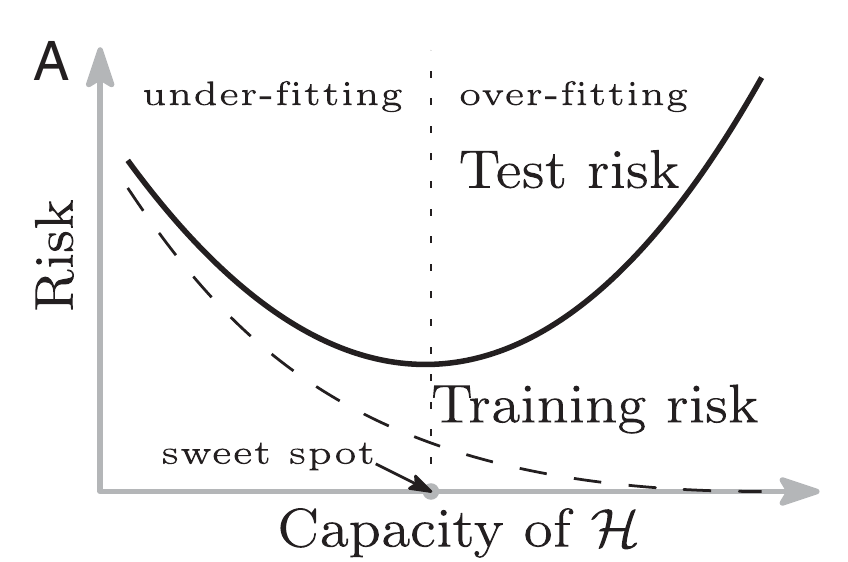
\includegraphics[height=6cm]{UCurve.png}
\\Classical curve from bias variance tradeoff.
\end{frame}

\begin{frame}
\frametitle{Modern practice}
\begin{itemize}
	\item Modern ML methods such as large neural networks and other non-linear predictors have very low to no training risk
	\item NN architectures chosen such that interpolation can be achieved.
	\item Works even when training data have high levels of noise.
\end{itemize}
\end{frame}

\begin{frame}
\frametitle{"Double Descent"}
Belkin proposed curve the extends beyond the poiny of interpolation
Observed empirically in a range of datasets
\end{frame}

\begin{frame}
\frametitle{Double Descent}
Graph picture, explain points of the graph.
\end{frame}

\begin{frame}
\frametitle{Double Descent}
Possible explanation by inductive bias and Occam's razor.
\end{frame}

\begin{frame}
\frametitle{Empirical Evidence}
RFFs. Might wanna explain more about RFFs approximating RKHS.
\end{frame}

\begin{frame}
\frametitle{Empirical Evidence}
Neural Networks. (Might be hard to explain why SGD is the inductive bias.)
\end{frame}

\begin{frame}
\frametitle{Historical absence}

\end{frame}

\begin{frame}
\frametitle{Appendix on Approximation Theorem}
On why they choose a function with a smaller norm in RKHS.
\end{frame}

\end{document} 
